%% Author: 端山和大

\subsection{重力波--電波マルチメッセンジャー観測} \label{transients.s3.gw}
近年、オーストラリアのParkes電波望遠鏡によりFRBと呼ばれる継続時間数msの突発的な電波天体が相次いで観測され (\Secref{transients.s1.frb})、日本でも \Figref{fig:transients.s3.gw.nasu}の那須電波観測所によって、数分から数日といったFRBより長いタイムスケールの突発天体 (WJN電波トランジェント; \Secref{transients.s3.unknowns}) が観測されている。
こういった電波帯域における突発天体は未だ対応天体が発見されておらず、その起源の解明はこれからの電波天文学にとって重要なテーマの一つである。
\begin{figure}
	\centering
	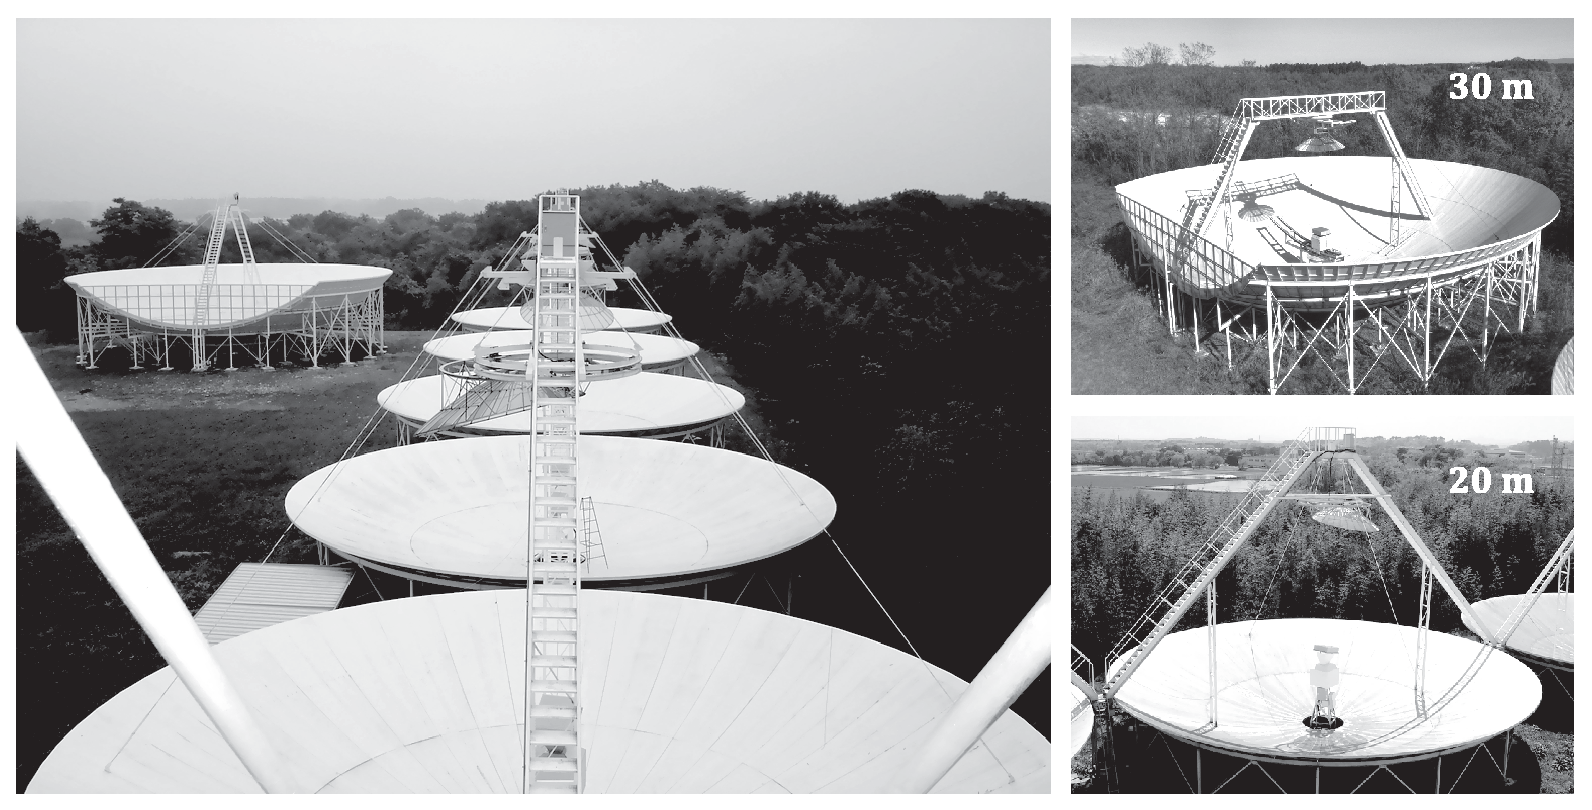
\includegraphics[width=1\textwidth]{transients/transients.s3.gw.nasu.eps}
	\caption{那須電波観測所。口径 20~m の電波望遠鏡8基、30~mの電波望遠鏡1基をもつ。}
	\label{fig:transients.s3.gw.nasu}
\end{figure}%

こうした突発天体は、そのエネルギーとタイムスケールから、重力波を伴うような天体爆発現象である可能性が示唆されている。
FRBのモデルとしては、重力波天体として最有力候補の一つである中性子連星合体時に起きるシンクロトロン放射\citep{2013PASJ...65L..12T}があり、またWJNイベントのモデルとしては、中性子星連星合体後に起きる電波アフターグローモデルが考えられる \citep{2011Natur.478...82N}。
さらに連星合体の際は、\Secref{transients.s1.grb}で述べたようにshort GRBも付随することが予想される。
そこで重力波と電波を中心とした、「マルチメッセンジャー観測」と呼ばれる多粒子・多波長による連携観測により、天体現象の多角的理解を目指す観測体制の構築が重要になる \citep{2012IAUS..285..331H}。

FRBの本来のイベントレートはおよそ$2 \times 10^4~\text{Gpc}^{-3}~\text{yr}^{-1}$ と見積もられており、現在建設中の重力波望遠鏡が見通せる、地球から$200~\text{Mpc}$ 以内で起こりうるFRBは、年間$160$ 個程度と考えられる。
このイベントレートは現在見積もられている連星中性子星合体のイベントレートの誤差範囲内にある。
もしFRBの起源が重力波天体であり、かつすべて検出できるならば、2020年には年間$160$程度の重力波--FRB同時観測が行われ、統計的な議論もできるようになると考えられる。
こうした突発天体を捉えるためには広い視野で長期間観測して天球上を走査することが最も有効になる。
SKAで採用が検討されている Phased Array Feed (PAF) は $18~\text{deg}^2$ という広い視野を持ち、\skasur{1} プログラムでは1年間で$550$時間、走査領域にして$10,000~\text{deg}^2$をカバーすることが予定されており、非常に有望な重力波マルチメッセンジャー観測体制を担う望遠鏡である。
さらにSKAでAdvanced Instrumentation Program (AIP) となっているMid-frequency Aperture Array (MAA) は、$200~\sqdeg$という驚異的な広視野を持ち、その実装は電波天文学のみならず重力波天文学にとっても極めて重要である。
